%\iffalse
\let\negmedspace\undefined
\let\negthickspace\undefined
\documentclass[journal,12pt,twocolumn]{IEEEtran}
\usepackage{cite}
\usepackage{amsmath,amssymb,amsfonts,amsthm}
\usepackage{algorithmic}
\usepackage{graphicx}
\usepackage{textcomp}
\usepackage{xcolor}
\usepackage{txfonts}
\usepackage{listings}
\usepackage{enumitem}
\usepackage{mathtools}
\usepackage{gensymb}
\usepackage{comment}
\usepackage[breaklinks=true]{hyperref}
\usepackage{tkz-euclide} 
\usepackage{listings}
\usepackage{gvv}                                        
\def\inputGnumericTable{}                                 
\usepackage[latin1]{inputenc}                                
\usepackage{color}                                            
\newtheorem{theorem}{Theorem}[section]
\usepackage{array}                                            
\usepackage{longtable}                                       
\usepackage{calc}                                             
\usepackage{multirow}                                         
\usepackage{hhline}                                           
\usepackage{ifthen}                                           
\usepackage{lscape}
\newtheorem{problem}{Problem}
\newtheorem{proposition}{Proposition}[section]
\newtheorem{lemma}{Lemma}[section]
\newtheorem{corollary}[theorem]{Corollary}
\newtheorem{example}{Example}[section]
\newtheorem{definition}[problem]{Definition}
\newcommand{\BEQA}{\begin{eqnarray}}
\newcommand{\EEQA}{\end{eqnarray}}
\newcommand{\define}{\stackrel{\triangle}{=}}
\theoremstyle{remark}
\newtheorem{rem}{Remark}
\begin{document}
\bibliographystyle{IEEEtran}
\vspace{3cm}
\title{NCERT: 10/5/3/18}
\author{EE23BTECH11040 - Manoj Kumar Ambatipudi$^{*}$% <-this % stops a space
}
\maketitle
\newpage
\bigskip
\renewcommand{\thefigure}{\theenumi}
\renewcommand{\thetable}{\theenumi}
\textbf{QUESTION:}
A spiral is made up of successive semi circles, with centres alternatively at A and B, Starting with center at A, of radii 0.5 cm, 1.0cm, 1.5cm, 2.0cm,... . What is the length of such a spiral ,made of 13 consecutive semicircles.(Use $\pi = \frac{22}{7}$) \\
\textbf{SOLUTION:}
\begin{table}[h]
\renewcommand\thetable{1}
    \centering
    \begin{tabular}{|c|c|c|}
    \hline
         Variables&Description&value  \\\hline
            $i_L\brak{0}$   &    Initial current in Inductor & 10A\\\hline
            L     & Inductance of Inductor & 0.5H\\\hline
    \end{tabular}
    \caption{Caption}
    \label{tab:EE_21_29_1}
\end{table}


General Term can be written as 
\begin{align}
    x\brak{n} = x\brak{0} + nd
\end{align}
Sum upto $n + 1$ terms is given by
\begin{align}
    y\brak{n} = x\brak{n}*u\brak{n}
\end{align}
The corresponding Z-Transform is given by \eqref{eq:APSum}.
Referring to \tabref{tab_10/5/3/18}, substituting the values in \eqref{eq:APSum}, 
\begin{align}
    Y\brak{z} = \frac{0.5}{\brak{1 - z^{-1}}^2} + \frac{0.5z^{-1}}{\brak{1-z^{-1}}^3} \quad ROC(\abs{z} > 1)
\end{align}
Finding $y\brak{n}$ by Contour Integration, 
\begin{align}
     y(12)&=\frac{1}{2\pi j}\oint_{C}\brak{\dfrac{0.5z^{12-1}}{\brak{1-z^{-1}}^2} + \dfrac{0.5z^{12-2}}{\brak{1-z^{-1}}^{3}}}dz  
\end{align}
Using Residue Theorem to evaluate the integral, let 
\begin{align}
    Y\brak{z} = S_{1} + S_{2}
\end{align}
$S_{1}$ has 2 poles,
\begin{align}
    S_{1} &= \frac{1}{\brak {1}!}\lim\limits_{z\to 1}\frac{d}{dz}\brak {{(z-1)}^{2}\frac{0.5z^{12+1}}{{(z-1)}^2}}\\
    S_{1} &= 0.5\brak{12+1}\lim\limits_{z\to 1}\brak{z^12}\\
    S_{1} &=0.5\brak{12+1}
\end{align}
Similarly, $S_{2}$ has 3 poles, 
\begin{align}
    S_{2}&=\frac{1}{\brak {2}!}\lim\limits_{z\to 1}\frac{d^{2}}{dz^{2}}\brak {{(z-1)}^{3}\frac{0.5z^{12+1}}{{(z-1)}^3}}\\
    &=\frac{0.5\brak{12+1}}{2}\lim\limits_{z\to 1}\frac{d}{dz}\brak{z^12}\\
    &=\frac{0.5\brak{12+1}\brak{12}}{2}\lim\limits_{z\to 1}\brak{z^{12-1}}\\
    &=\frac{0.5\brak{12}\brak{12+1}}{2}
\end{align}
Finally, 
\begin{align}
    y\brak{12} &= 0.5\brak{12+1} + \frac{0.5\brak{12}\brak{12+1}}{2}\\
    y\brak{12} &= 45.5
\end{align}
\begin{align}
    \sum_{n = 0}^{12}C_{n} &= \pi y\brak{12}\\
    \sum_{n = 0}^{12}C_{n} &= \pi \brak{45.5}\\
                           &= 143
\end{align}

\begin{figure}[h]
\renewcommand\thefigure{1}
    \centering
    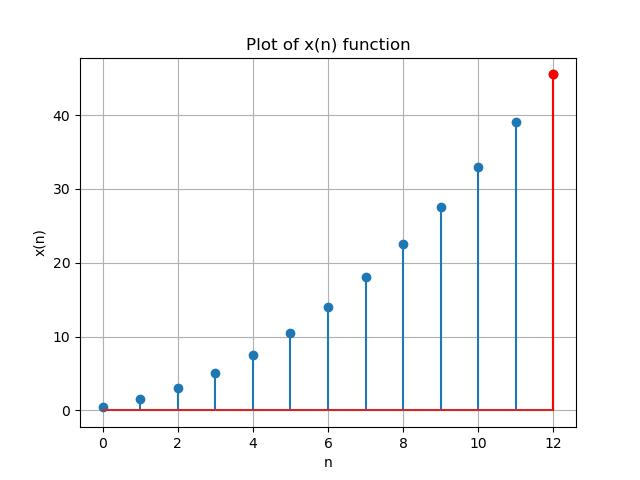
\includegraphics[width=1.0\columnwidth]{figs/fig_1.jpg}
    \caption{Plot of Sum of $n$ terms taken from Python3}
    \label{fig_2}
\end{figure}
\end{document}  

